\documentclass[11pt]{article}
\usepackage[utf8]{inputenc}
\usepackage[T1]{fontenc}
\usepackage{geometry}
\usepackage{amsmath,amssymb,amsthm}
\usepackage{algorithm}
\usepackage{algorithmic}
\usepackage{graphicx}
\usepackage{subcaption}
\usepackage{booktabs}
\usepackage{array}
\usepackage{multirow}
\usepackage{longtable}
\usepackage{rotating}
\usepackage{pdflscape}
\usepackage{afterpage}
\usepackage{capt-of}
\usepackage{float}
\usepackage{hyperref}
\usepackage{cleveref}
\usepackage{listings}
\usepackage{xcolor}
\usepackage{tikz}
\usepackage{pgfplots}
\pgfplotsset{compat=1.17}

\geometry{margin=1in}

% Custom colors
\definecolor{codegreen}{rgb}{0,0.6,0}
\definecolor{codegray}{rgb}{0.5,0.5,0.5}
\definecolor{codepurple}{rgb}{0.58,0,0.82}
\definecolor{backcolour}{rgb}{0.95,0.95,0.92}

% Code listing style
\lstdefinestyle{mystyle}{
    backgroundcolor=\color{backcolour},
    commentstyle=\color{codegreen},
    keywordstyle=\color{magenta},
    numberstyle=\tiny\color{codegray},
    stringstyle=\color{codepurple},
    basicstyle=\ttfamily\footnotesize,
    breakatwhitespace=false,
    breaklines=true,
    captionpos=b,
    keepspaces=true,
    numbers=left,
    numbersep=5pt,
    showspaces=false,
    showstringspaces=false,
    showtabs=false,
    tabsize=2
}
\lstset{style=mystyle}

% Title information
\title{\textbf{Sports Tournament Scheduling: \\
A Multi-Paradigm Optimization Approach}}

\author{
Leonardo Tassinari, leonardo.tassinari6@studio.unibo.it
\\
Francesco Zattoni, francesco.zattoni2@studio.unibo.it
\\ 
}

\date{July 2025}

\begin{document}

\maketitle

\section{Introduction}
This report presents a comprehensive study of the Sports Tournament Scheduling (STS) problem, focusing on the development and comparison of multiple optimization models. The aim is to provide a unified framework for modeling, analyzing, and solving the STS problem, enabling a fair and systematic evaluation of different solution paradigms. All models considered in this work share a common formalization, which is described in this section.\\
The repository is available at \url{https://github.com/leo-tasso/STS}.

\subsection{Common Model Formalization}

\paragraph{Input Parameters.}
The STS problem is defined by the following parameters, which are common to all models:
\begin{itemize}
    \item $n$: Number of teams (even integer)
    \item $w = n-1$: Number of weeks
    \item $p = n/2$: Number of periods (matches per week)
    \item Teams are indexed by $t \in \{1, 2, \ldots, n\}$
    \item Weeks are indexed by $w \in \{1, 2, \ldots, n-1\}$
    \item Periods are indexed by $p \in \{1, 2, \ldots, n/2\}$
\end{itemize}

\paragraph{Objective Variable and Bounds.}
For the optimization variant, the objective is to minimize the maximum imbalance in home and away games for any team:
\[
M = \max_{t \in \{1, \ldots, n\}} |h_t - a_t|
\]
where $h_t$ and $a_t$ denote the number of home and away games played by team $t$, respectively. The upper bound for $M$ is $n-1$, even if the practical upper bound is lower, because it's impossible that every team plays only away games or home games. The theoretical lower bound for $M$ is $1$ for even $n$, since $h_t$ and $a_t$ cannot be equal.

\paragraph{Constraints.}
All models enforce the following core constraints:
\begin{enumerate}
    \item Each pair of teams plays exactly once during the tournament.
    \item Each team plays exactly once per week.
    \item Each period in each week hosts exactly one match.
    \item No team plays against itself.
    \item Each team appears in the same period at most twice across all weeks.
\end{enumerate}

\paragraph{Pre-processing and Symmetry Breaking.}
To improve solver efficiency, all models may include pre-processing steps such as:
\begin{itemize}
    \item Translating the model into a solver-independent language (such as DIMACS or SMT-LIB), which may require additional pre-processing time before the actual solving phase. 
    \item Fixing the schedule of the first week to break team symmetries.
    \item Lexicographic ordering of weeks and/or periods to break week and period symmetries.
    \item Adding implied constraints (e.g., total matches per team).
\end{itemize}

\paragraph{Validation}
Each test is executed five times, using a timeout of 300 seconds, on the same hardware: a Ryzen 5 5600X CPU with 32 GB of RAM, running inside a Docker container based on Ubuntu 22.04. Different solvers and approaches are evaluated, including variations in active constraints. The result tables report both the time in seconds taken for the decision version and the objective value found where the optimization version is used (CP, Z3 both SAT and SMT, MIP). Each cell contains \texttt{decision\_seconds}|\texttt{opt\_obj\_value}, if an optimization version is defined, otherwise only the \texttt{decision\_seconds}.

\section{CP model}

\subsection{Decision Variables}

The MiniZinc CP model represents the tournament schedule using two primary arrays of integer decision variables:

\begin{itemize}
    \item \texttt{home[$w$, $p$]}: For each week $w$ and period $p$, \texttt{home[$w$, $p$]} is an integer variable indicating the team assigned as the home team in that slot.
    \item \texttt{away[$w$, $p$]}: For each week $w$ and period $p$, \texttt{away[$w$, $p$]} is an integer variable indicating the team assigned as the away team in that slot.
\end{itemize}

Both variables take values in $\{1, \ldots, n\}$ and together define the assignment of teams to each match in the tournament schedule. All additional variables and constraints in the model are defined in terms of these primary decision variables, as described in the common formalization. \\
Another design of the decision variables was tested: \texttt{matches}, an array for each possible match ID that takes values in $\{1..slots\},\ slots = (n-1)\times(n/2)$, but it led to a more complex implementation with not-so-evident improvements only for $n=12$. Also, the addition of channeling constraints between \texttt{matches}, \texttt{home} and \texttt{away} didn't help.

\subsection{Objective Function}

The objective variable and its theoretical bounds are described in Section~1. In the MiniZinc model, the objective is implemented as the variable \texttt{max\_diff}, which represents the maximum absolute difference between the number of home and away games for any team:
\[
\texttt{max\_diff} = \max_{t \in \text{Teams}} \left|\,\texttt{home\_count}[t] - \texttt{away\_count}[t]\,\right|
\]
where the auxiliary variables \texttt{home\_count}[t] and \texttt{away\_count}[t] are defined as follows:
\begin{itemize}
    \item \texttt{home\_count}[t]: the total number of times team $t$ appears as the home team across all weeks and periods,
    \[
    \texttt{home\_count}[t] = \sum_{w \in \text{Weeks}} \sum_{p \in \text{Periods}} [\texttt{home}[w,p] = t]
    \]
    \item \texttt{away\_count}[t]: the total number of times team $t$ appears as the away team across all weeks and periods,
    \[
    \texttt{away\_count}[t] = \sum_{w \in \text{Weeks}} \sum_{p \in \text{Periods}} [\texttt{away}[w,p] = t]
    \]
\end{itemize}

The auxiliary variables \texttt{home\_count}[t] and \texttt{away\_count}[t] are computed efficiently using the \texttt{global\_cardinality} constraint in MiniZinc.

The model minimizes \texttt{max\_diff} using the following directive:
\begin{verbatim}
solve minimize max_diff;
\end{verbatim}

\subsection{Constraints}

\paragraph{Main Problem Constraints}

\begin{itemize} 
    \item \textbf{Each pair of teams plays exactly once.}  
    For every unordered pair of distinct teams $(i, j)$, there must be exactly one match where $i$ plays against $j$ (either as home or away):
    \begin{equation*}
        \sum_{w \in \text{Weeks}} \sum_{p \in \text{Periods}} \left( [\texttt{home}[w,p] = i \land \texttt{away}[w,p] = j] + [\texttt{home}[w,p] = j \land \texttt{away}[w,p] = i] \right) = 1
    \end{equation*}

    \item \textbf{Each team plays exactly once per week.}  
    In every week $w$, each team must appear exactly once, either as home or away. This is enforced by requiring that all teams assigned in week $w$ are distinct:
    \begin{equation*}
        \text{The set } \{\texttt{home}[w,p],\ \texttt{away}[w,p] : p \in \text{Periods}\} \text{ contains all teams without repetition.}
    \end{equation*}
    This constraint is implemented using \texttt{all\_different} for every week $w$.

    \item \textbf{Each team appears in the same period at most twice.}  
    To model this constraint, we define the variable \texttt{period\_count}[t, p] as follows:
    \begin{equation*}
        \texttt{period\_count}[t, p] = \sum_{w \in \text{Weeks}} \left( [\texttt{home}[w,p] = t] + [\texttt{away}[w,p] = t] \right)
    \end{equation*}
    This expression is implemented in MiniZinc using the \texttt{global\_cardinality} constraint, used to enforce the final constraint as:
    \begin{equation*}
        \texttt{period\_count}[t, p] \leq 2
    \end{equation*}
\end{itemize}


\paragraph{Implied Constraints}
These constraints are semantically redundant, but they can be useful to reduce the search space.

\begin{itemize}
    \item \textbf{Total matches per team:}  
    Each team $t$ must play exactly $n-1$ matches in total (as home or away):
    \begin{equation*}
        \texttt{home\_count}[t] + \texttt{away\_count}[t] = n - 1
    \end{equation*}

    \item \textbf{Total period appearances per team:}  
    Each team $t$ must appear in some period exactly $n - 1$ times over the tournament, exploiting the previously defined variable \texttt{period\_count}:
    \begin{equation*}
        \sum_{p \in \text{Periods}} \texttt{period\_count}[t, p] = n - 1
    \end{equation*}
\end{itemize}

\paragraph{Symmetry Breaking Constraints}

The STS problem exhibits several symmetries (e.g., relabeling teams, reordering weeks or periods) that can lead to redundant search. Symmetry breaking constraints reduce the number of equivalent solutions and improve solver efficiency:

\begin{itemize}
    \item \textbf{Week symmetry:}  
    Weeks can be permuted without changing the problem. To break this symmetry, we impose lexicographic ordering between consecutive weeks:
    \begin{equation*}
        (\texttt{home}[w,1], \ldots, \texttt{home}[w,p], \texttt{away}[w,1], \ldots, \texttt{away}[w,p]) <_{\text{lex}} (\texttt{home}[w+1,1], \ldots, \texttt{away}[w+1,p])
    \end{equation*}
    for all $w \in \{1, 2, \ldots, n-2\}$.

    \item \textbf{Period symmetry:}  
    Periods within a week can be permuted. We enforce lexicographic ordering between periods:
    \begin{equation*}
        (\texttt{home}[1,p], \ldots, \texttt{home}[w,p], \texttt{away}[1,p], \ldots, \texttt{away}[w,p]) <_{\text{lex}} (\texttt{home}[1,p+1], \ldots, \texttt{away}[w,p+1])
    \end{equation*}
    for all $p \in \{1, 2, \ldots, n/2-1\}$.

    \item \textbf{Team symmetry:}  
    Teams can be relabeled. We fix the first week schedule to a canonical order:
    \begin{equation*}
        \texttt{home}[1, i] = 2i - 1,\quad \texttt{away}[1, i] = 2i
    \end{equation*}
    for all $p$ in periods.
    \\
    This approach was already used for a similar problem, as shown in \cite{teamsymm}.
\end{itemize}

\subsection{Validation}

To validate the MiniZinc model, we conducted a systematic experimental study using two different solvers: \textbf{Gecode} and \textbf{Chuffed}. Both solvers were run on the same set of problem instances to allow for a fair comparison. The experiments were designed to assess the impact of symmetry breaking and implied constraints, as well as the effect of different search strategies.

\paragraph{Experimental Design}
The validation of the MiniZinc model was performed using the two already mentioned solvers with common search strategies: \texttt{first\_fail} heuristic to select the variable with the smallest domain, \texttt{relax\_and\_reconstruct(85)} to escape local minima by fixing $85\%$ of the found solution and reconstructing the remaining part of it. \\One search strategy differs per solver: Gecode employed also the \texttt{indomain\_random} to assign a randomly chosen value from the selected variable; Chuffed was tested using \texttt{indomain\_min}, as \texttt{indomain\_random} is not supported. \\
Restart strategies were tested only with Chuffed, even though it did not use \texttt{indomain\_random}, because applying any restart strategy with Gecode led to worse performance. Among the strategies tested, \texttt{restart\_luby} showed the best performance in previous experiments and was therefore selected for the final tests. \\
Experiments were conducted on MiniZinc 2.9.3 with Gecode 6.3.0 and Chuffed 0.13.2.\\
For each instance, we evaluated the following configurations:
\begin{itemize}
    \item Chuffed and Gecode with/without symmetry breaking constraints,
    \item Chuffed and Gecode with/without implied constraints,
    \item Chuffed and Gecode with/without search strategies.
\end{itemize} 
Also, other strategies were used, but they didn't improve either the performance or the complexity of the implemented model: we tried \texttt{bounds} and \texttt{domain} to make the solver use specific kinds of constraint propagation; a change in the order of the variables, i.e. swapping the weeks with the periods in both \texttt{home} and \texttt{away} arrays.

\paragraph{Experimental Results}

The results obtained using the described search strategies are reported in the following tables and in the plot to assess the effectiveness of symmetry breaking constraints, implied constraints, and search strategies. In the table \ref{tab:cp}, C. stands for Chuffed and G. stands for Gecode.

\begin{table}[H]
\small
\begin{tabular}{@{}lcccccccc@{}}
\toprule
ID & C. (all) & C. w/o SB & C. w/o IC & C. w/o SS & G. (all) & G. w/o SB & G. w/o IC & G. w/o SS \\
\midrule
6 & 0 | \textbf{1} & 0 | \textbf{1} & 0 | \textbf{1} & 0 | \textbf{1} & 0 | \textbf{1} & 0 | \textbf{1} & 0 | \textbf{1} & 0 | \textbf{1}\\
8 & 0 | \textbf{1} & 0 | \textbf{1} & 0 | \textbf{1} & 0 | \textbf{1} & 1 | \textbf{1} & 9 | \textbf{1} & 73 | \textbf{1} & 2 | \textbf{1}\\
10 & 3 | \textbf{1} & 4 | \textbf{1} & 3 | \textbf{1} & 3 | \textbf{1} & 8 | \textbf{1} & 63 | \textbf{1} & 146 | \textbf{1} & \texttt{N/A} | \textbf{\texttt{N/A}}\\
12 & 110 | \textbf{3} & 16 | \textbf{1} & 56 | \textbf{5} & 109 | \textbf{5} & \texttt{N/A} | \textbf{\texttt{N/A}} & \texttt{N/A} | \textbf{\texttt{N/A}} & \texttt{N/A} | \textbf{\texttt{N/A}} & \texttt{N/A} | \textbf{\texttt{N/A}}\\
14 & \texttt{N/A} | \textbf{\texttt{N/A}} & 37 | \textbf{13} & \texttt{N/A} | \textbf{\texttt{N/A}} & \texttt{N/A} | \textbf{\texttt{N/A}} & \texttt{N/A} | \textbf{\texttt{N/A}} & \texttt{N/A} | \textbf{\texttt{N/A}} & \texttt{N/A} | \textbf{\texttt{N/A}} & \texttt{N/A} | \textbf{\texttt{N/A}}\\
16 & \texttt{N/A} | \textbf{\texttt{N/A}} & \texttt{N/A} | \textbf{15} & \texttt{N/A} | \textbf{\texttt{N/A}} & \texttt{N/A} | \textbf{\texttt{N/A}} & \texttt{N/A} | \textbf{\texttt{N/A}} & \texttt{N/A} | \textbf{\texttt{N/A}} & \texttt{N/A} | \textbf{\texttt{N/A}} & \texttt{N/A} | \textbf{\texttt{N/A}}\\
\bottomrule
\end{tabular}
\caption{Results using Chuffed (C.) and Gecode (G.) with the possible combinations of active constraints, both in decision and optimization version.}
\label{tab:cp}
\end{table}

\begin{figure}[H]
    \centering
    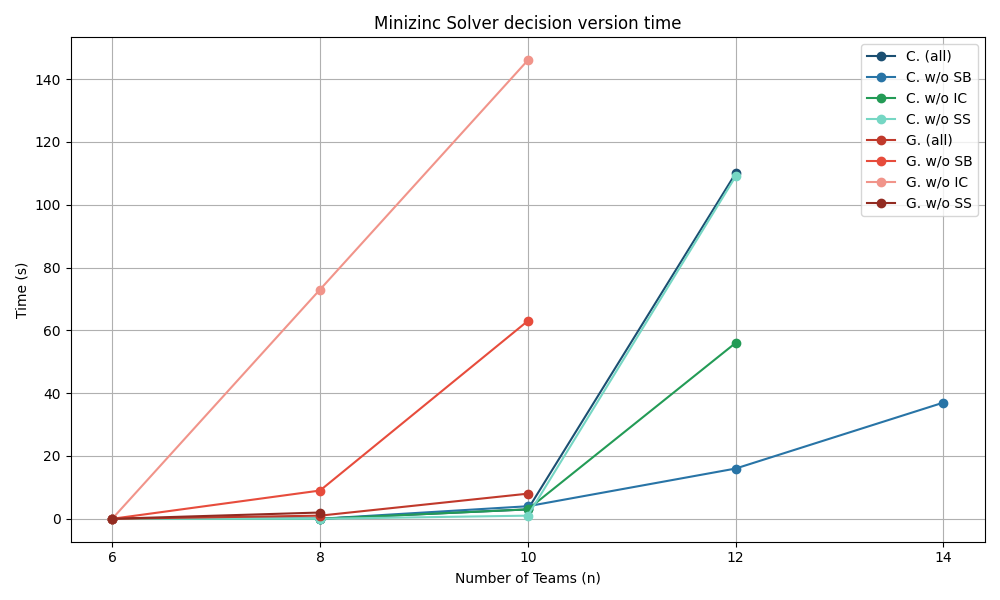
\includegraphics[width=0.8\textwidth]{cp_plot.png}
    \caption{Minizinc solvers: solving time for different constraint configurations.}
    \label{fig:cp_plot}
\end{figure}

\section{SAT Model}

\subsection{Decision variables}
The core decision variables in the SAT model are 3D arrays: 
\begin{itemize}
    \item \texttt{home[$w$, $p$, $t$]}: Boolean variables where \texttt{home[$w$, $p$, $t$]} is true if and only if team $t$ plays at home in week $w$ during period $p$.

\texttt{away[$w$, $p$, $t$]}: Boolean variables where \texttt{away[$w$, $p$, $t$]} is true if and only if team $t$ plays away in week $w$ during period $p$.
\end{itemize}
Other auxiliary variables are added for the encodings of the cardinality constraints, that will be discussed in Section~3.3.

\subsection{Objective Function}

To optimize an objective function in SAT we use a \emph{binary search} approach over possible values of the objective. For each candidate value, we encode the constraint ``no team has a home/away imbalance greater than $d$'' as SAT clauses, and check satisfiability.
\\The objective is:
\[
\min \max_{t} |H_t - A_t|
\]
Since $H_t + A_t = w$ for all $t$, minimizing $|H_t - A_t|$ is equivalent to bounding $H_t$ within $[\lfloor w/2 \rfloor - d/2, \lceil w/2 \rceil + d/2]$ for some $d$.
\\
The sum $H_t = \sum_{w,p} \texttt{home[$w$, $p$, $t$]}$ is the number of home games for team $t$.
To enforce the objective, for a given candidate $d$, we add for each team $t$:
\[
\texttt{min\_home} \leq H_t \leq \texttt{max\_home}
\]
where
\[
\texttt{min\_home} = \max\left(0, \frac{w - d}{2}\right), \quad
\texttt{max\_home} = \min\left(w, \frac{w + d}{2}\right)
\]
During the binary search, $d$ becomes smaller, approaching $1$, then \texttt{min\_home} and \texttt{max\_home} approach $w/2$, leading to a more balanced scheduling.

\subsection{Constraints}

\paragraph{Main Problem Constraints}
\begin{itemize}
    \item \textbf{Each slot has exactly one home and one away team, and they are different:}
    \begin{align}
        &\forall w, p: \quad \texttt{exactly\_one}(\{\forall t: \space \texttt{home[$w$, $p$, $t$]}\}) \\
        &\forall w, p: \quad \texttt{exactly\_one}(\{\forall t: \space \texttt{away[$w$, $p$, $t$]}\}) \\
        &\forall w, p, t: \quad \texttt{home[$w$, $p$, $t$]} \implies \neg \texttt{away[$w$, $p$, $t$]}
    \end{align}
    This ensures each slot is filled by one home and one away team, and a team cannot be both in the same slot.

    \item \textbf{Each pair of teams plays exactly once:}
    \begin{align}
        &\forall i < j: \quad \texttt{exactly\_one}(\{ \forall w, p: \space \texttt{home[$w$, $p$, $i$]} \land \texttt{away[$w$, $p$, $j$]}, \texttt{home[$w$, $p$, $j$]} \land \texttt{away[$w$, $p$, $i$]}\})
    \end{align}
    This ensures every pair of teams meets exactly once, with one as home and one as away.

    \item \textbf{Each team plays once per week:}
    \begin{align}
        &\forall w, t: \quad \texttt{exactly\_one}(\{\forall p: \space \texttt{home[$w$, $p$, $t$]}, \texttt{away[$w$, $p$, $t$]}\})
    \end{align}
    Each team appears in exactly one match per week.

    \item \textbf{Period limit: Each team appears in the same period at most twice:}
    \begin{align}
        &\forall t, p: \quad \texttt{at\_most\_k}(\{\forall w: \texttt{home[$w$, $p$, $t$]}, \texttt{away[$w$, $p$, $t$]}\}, 2)
    \end{align}
    No team is scheduled in the same period more than twice.
\end{itemize}

\paragraph{Implied Constraints}
\begin{itemize}
    \item \textbf{Number of games per team:}
    \begin{align}
        &\forall t: \quad \texttt{exactly\_k}(\{\forall w,p: \texttt{home[$w$, $p$, $t$]}, \texttt{away[$w$, $p$, $t$]}\}, n-1)
    \end{align}
    Each team plays $n-1$ games (one per week).

    \item \textbf{Total period appearances:}
    \begin{align}
        &\forall t: \quad \texttt{exactly\_k}(\{\forall w,p: \space \texttt{home[$w$, $p$, $t$]}, \texttt{away[$w$, $p$, $t$]}\}, n-1)
    \end{align}
    Each team appears in periods a total of $n-1$ times.
\end{itemize}

\paragraph{Symmetry Breaking Constraints}
The lexicographical order constraints used in the CP model are enforced only on the first pair of weeks and periods, because applying them on the whole schedule would lead to an explosion of constraints and to an overall time performance decrease.
\begin{itemize}
    \item \textbf{Weeks:} Lexicographically order the first two weeks to break symmetry:
\begin{align}
    &\texttt{lex\_less}(
        [\forall t, p:\space\texttt{home[$0$, $p$, $t$]}, \texttt{away[$0$, $p$, $t$]}], \\
    &\quad\quad\quad\quad
        [\forall t, p: \texttt{home[$1$, $p$, $t$]}, \texttt{away[$1$, $p$, $t$]}]
    )
\end{align}

\item \textbf{Periods:} Lexicographically order the first two periods to break symmetry:
\begin{align}
    &\texttt{lex\_less}(
        [\forall w, t : \texttt{home[$w$, $0$, $t$]}, \texttt{away[$w$, $0$, $t$]}], \\
    &\quad\quad\quad\quad
        [\forall w, t: \texttt{home[$w$, $1$, $t$]}, \texttt{away[$w$, $1$, $t$]}]
    )
\end{align}


    \item \textbf{Teams:} Fix the assignment in the first week:
    \begin{align}
        &\forall i: \quad \texttt{home[$0$, $i$, $2i$]} \land \texttt{away[$0$, $i$, $2i+1$]}
    \end{align}
    This removes equivalent solutions due to team relabeling.
\end{itemize}


\paragraph{Encoding Methods}
\begin{itemize}
    \item \textbf{Exactly-one, at-most-k, and exactly-k constraints:} These are encoded using various SAT encodings, selectable in the CLI by the user:
    \begin{itemize}
        \item \texttt{np}: Naive pairwise encoding.
        \item \texttt{seq}: Sequential counter encoding (used for at-most-k and exactly-k).
        \item \texttt{bw}: Bitwise encoding for exactly-one.
        \item \texttt{he}: Heule encoding for exactly-one.
    \end{itemize}
    The sequential counter encoding is used for cardinality constraints (at-most-k, at-least-k, exactly-k) for efficiency. Indeed, in Section~3.4 the validation results report only the ones given the best encoding methods, i.e. the bitwise one for the cardinality constraints with $k=1$ and the sequential one for constraints with $k>1$.
\end{itemize}

\subsection{Validation}

\paragraph{Model Validation with Z3.}
The primary implementation of the STS model uses the Z3 SMT solver. All constraints are encoded as Z3 Boolean formulas, and the model is validated by checking satisfiability and extracting a solution using Z3's API.

\paragraph{Solver-Independent Validation via DIMACS.} The Z3 model can also be exported to the standard DIMACS CNF format, which is supported by most SAT solvers. This is achieved by:
\begin{itemize}
    \item Using Z3's \texttt{tseitin-cnf} tactic \cite{tseitin} to convert the Z3 Boolean model into CNF.
    \item Exporting the CNF to DIMACS format, including variable mappings, i.e. the mapping from the assigned integer value to the Z3 boolean variable.
    \item Parsing the DIMACS file and solving it with external SAT solvers (e.g., Minisat, Glucose) via the PySAT library.
    \item Decoding the resulting model back into the tournament schedule using the variable mappings.
\end{itemize}
This approach allows the same model to be validated with different SAT solvers, ensuring correctness and robustness of the encoding.

\paragraph{Experimental Results} The following tables and plot show the time performance of the different solvers given the best encoding method:
\begin{table}[H]
\centering
\small
\label{tab:z3}
\begin{tabular}{@{}lcccc@{}}
\toprule
ID & Z3 (all) & Z3 w/o SB & Z3 w/o IC \\
\midrule
6 & 0 | \textbf{1} & 0 | \textbf{1} & 0 | \textbf{1} \\
8 & 2 | \textbf{1} & 2 | \textbf{1} & 0 | \textbf{1}  \\
10 & 8 | \textbf{1} & 10 | \textbf{5} & 1 | \textbf{1} \\
12 & \texttt{N/A} | \textbf{6} & \texttt{N/A} | \textbf{6} & \texttt{N/A} | \textbf{6} \\
\bottomrule
\end{tabular}
\caption{Results using Z3 with the possible combinations of active constraints.}
\end{table}

\begin{table}[H]
\centering
\small
\label{tab:glucosems}
\begin{tabular}{@{}lccccccc@{}}
\toprule
ID & G. (all) & G. w/o SB & G. w/o IC & M.S. (all) & M.S. w/o SB & M.S. w/o IC\\
\midrule
6 & 0 & 0 & 0 & 0 & 0 & 0\\
8 & 0 & 1 & 0 & 0 & 1 & 0 \\
10 & 4 & 72 & 2 & 4 & 48 & 5\\
12 & 116 & \texttt{N/A} & 132 & 49 & \texttt{N/A} & 281\\
\bottomrule
\end{tabular}
\caption{Results using Glucose (G.) and MiniSAT (M.S.) with the possible combinations of active constraints.}
\end{table}

\begin{figure}[H]
    \centering
    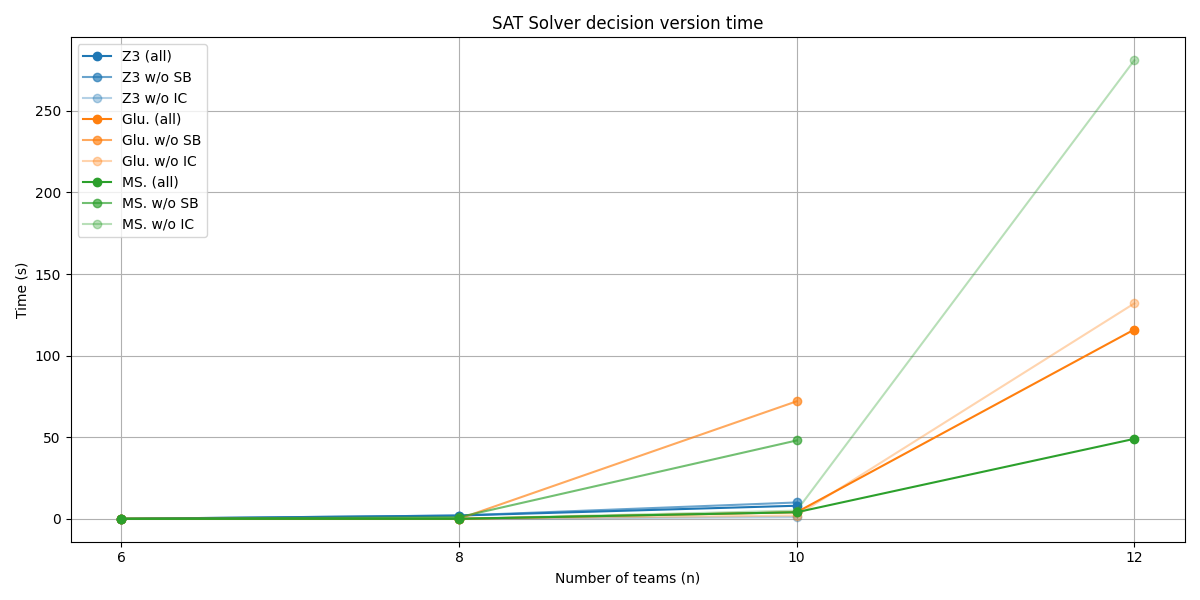
\includegraphics[width=0.7\textwidth]{sat_plot.png}
    \caption{SAT solvers: solving time for different constraint configurations.}
    \label{fig:sat_plot}
\end{figure}

\section{SMT Model}

\subsection{Decision Variables}

The SMT model employs integer decision variables that naturally express the tournament structure. All variables are defined over the integer sort using the theory of linear integer arithmetic (LIA):

\begin{align}
    \forall w, p:\space\texttt{home}[w,p] &: \textbf{Int}, \quad 1 \leq \texttt{home}[w,p] \leq n \\
    \forall w, p:\space\texttt{away}[w,p] &: \textbf{Int}, \quad 1 \leq \texttt{away}[w,p] \leq n
\end{align}

where $\texttt{home}[w,p]$ represents the team playing at home in week $w$, period $p$, and $\texttt{away}[w,p]$ represents the team playing away in the same slot.

\textbf{Auxiliary variables:}
\begin{align}
\forall t:\space\texttt{home\_count}[t] &: \textbf{Int}  \\
\forall t:\space\texttt{away\_count}[t] &: \textbf{Int}  \\
\texttt{max\_diff} &: \textbf{Int}
\end{align}

\subsection{Objective Function}

The objective function minimizes the maximum home/away imbalance across all teams. In SMT, this is expressed using optimization assertions:

\begin{align}
\textbf{minimize } \texttt{max\_diff}
\end{align}

where $\texttt{max\_diff}$ is constrained as:
\begin{align}
\forall t: \quad \texttt{max\_diff} \geq |\texttt{home\_count}[t] - \texttt{away\_count}[t]| \Rightarrow \\
\texttt{max\_diff} = \max_{t} |\texttt{home\_count}[t] - \texttt{away\_count}[t]|
\end{align}

The above defined objective function is inserted only in the Z3 solver, since SMT-LIB does not support natively the optimization.

\subsection{Constraints}

All constraints are expressed using the theory of linear integer arithmetic (LIA).

\paragraph{Main Problem Constraints}
\begin{itemize}
    \item \textbf{No team plays against itself:}
    \begin{align}
        \forall w, p: \quad \texttt{home}[w,p] \neq \texttt{away}[w,p]
    \end{align}

    \item \textbf{Each team plays exactly once per week:}
    \begin{align}
        \forall w: \quad
        \textbf{distinct}(\texttt{home}[w,1], \ldots, \texttt{home}[w,n/2], \texttt{away}[w,1], \ldots, \texttt{away}[w,n/2])
    \end{align}

    \item \textbf{Each pair of teams plays exactly once:}
    \begin{align}
        \forall i, j \text{ with } i < j: \quad
        &\sum_{w=1}^{n-1} \sum_{p=1}^{n/2} \Big( \textbf{ite}(\texttt{home}[w,p] = i \land \texttt{away}[w,p] = j, 1, 0) \nonumber \\
        &\qquad\qquad + \textbf{ite}(\texttt{home}[w,p] = j \land \texttt{away}[w,p] = i, 1, 0) \Big) = 1
    \end{align}

    \item \textbf{Period limit constraint:}
    \begin{align}
        \forall t, p: \quad
        \sum_{w=1}^{n-1} \left( \textbf{ite}(\texttt{home}[w,p] = t, 1, 0) + \textbf{ite}(\texttt{away}[w,p] = t, 1, 0) \right) \leq 2
    \end{align}
\end{itemize}

\paragraph{Auxiliary Variable Definitions}
\begin{align}
\forall t: \quad \texttt{home\_count}[t] &= \sum_{w=1}^{n-1} \sum_{p=1}^{n/2} \textbf{ite}(\texttt{home}[w,p] = t, 1, 0) \\
\forall t: \quad \texttt{away\_count}[t] &= \sum_{w=1}^{n-1} \sum_{p=1}^{n/2} \textbf{ite}(\texttt{away}[w,p] = t, 1, 0)
\end{align}

\paragraph{Implied Constraints}
\begin{itemize}
    \item \textbf{Total matches per team:}
    \begin{align}
        \forall t: \quad \texttt{home\_count}[t] + \texttt{away\_count}[t] = n - 1
    \end{align}

    \item \textbf{Total period appearances:}
    \begin{align}
        \forall t: \quad
        \sum_{p=1}^{n/2} \sum_{w=1}^{n-1} \left( \textbf{ite}(\texttt{home}[w,p] = t, 1, 0) + \textbf{ite}(\texttt{away}[w,p] = t, 1, 0) \right) = n - 1
    \end{align}
\end{itemize}

\paragraph{Symmetry Breaking Constraints}
\begin{itemize}
    \item \textbf{Team symmetry:}
    \begin{align}
        \forall p: \quad \texttt{home}[1,p] &= 2p - 1 \\
        \forall p: \quad \texttt{away}[1,p] &= 2p
    \end{align}

    \item \textbf{Lexicographic ordering for weeks:}
    \begin{align}
        \forall w: \quad
        &(\texttt{home}[w,1], \ldots, \texttt{home}[w,n/2], \texttt{away}[w,1], \ldots, \texttt{away}[w,n/2]) \\
        &\quad <_{\textbf{lex}} (\texttt{home}[w+1,1], \ldots, \texttt{home}[w+1,n/2], \texttt{away}[w+1,1], \ldots, \texttt{away}[w+1,n/2]) \nonumber
    \end{align}

    \item \textbf{Lexicographic ordering for periods:}
    \begin{align}
        \forall p: \quad
        &(\texttt{home}[1,p], \ldots, \texttt{home}[n-1,p], \texttt{away}[1,p], \ldots, \texttt{away}[n-1,p]) \\
        & <_{\textbf{lex}} (\texttt{home}[1,p+1], \ldots, \texttt{home}[n-1,p+1], \texttt{away}[1,p+1], \ldots, \texttt{away}[n-1,p+1]) \nonumber
    \end{align}
\end{itemize}

\subsection{Validation}

The SMT model was implemented using both Z3 and CVC5 solvers to ensure robustness and enable solver comparison. To enable a solver-independent comparison, the model was also encoded in SMT-LIB format.

\paragraph{Experimental Results}

The SMT model was validated with both Z3 and CVC5 for the decision version and Z3 only for the optimization one:

\begin{table}[H]
\centering
\small
\label{tab:smt}
\begin{tabular}{@{}lccccccc@{}}
\toprule
ID & Z3 (all) & Z3 w/o SB & Z3 w/o IC & CVC5 (all) & CVC5 w/o SB & CVC5 w/o IC \\
\midrule
6 & 0 | \textbf{1} & 0 | \textbf{1} & 0 | \textbf{1} &  0 | &  1 | &  0 |\\
8 & 0 | \textbf{1} & 2 | \textbf{1} & 0 | \textbf{1} & 18 | & 33 | & 20 |\\
10 &  30 | \texttt{N/A} &  49 | \texttt{N/A} &  37 | \texttt{N/A} & \texttt{N/A} | & \texttt{N/A} | & \texttt{N/A} |\\
12 &  216 | \texttt{N/A} &  289 | \texttt{N/A} & \texttt{N/A} | \texttt{N/A} & \texttt{N/A} | & \texttt{N/A} | & \texttt{N/A} |\\
\bottomrule
\end{tabular}
\caption{Results using Z3 and CVC5 with the possible combinations of active constraints.}
\end{table}

\begin{figure}[H]
    \centering
    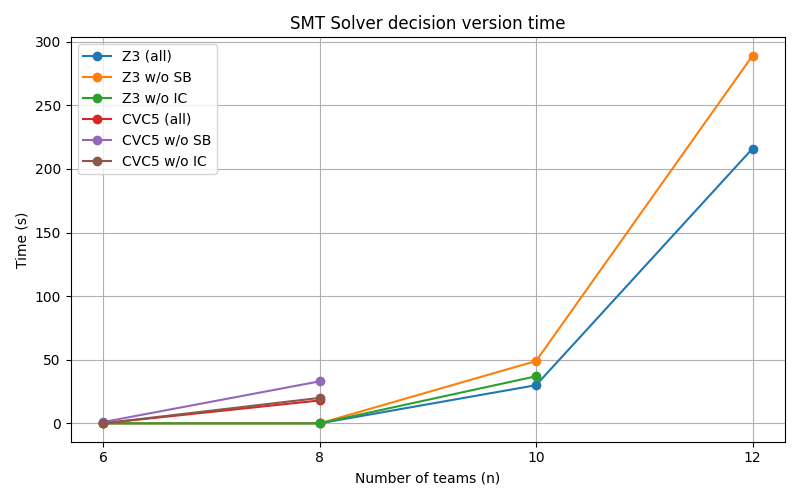
\includegraphics[width=0.7\textwidth]{SMT_solvers.png}
    \caption{SMT solvers: solving time for different constraint configurations.}
    \label{fig:smt_plot}
\end{figure}

\section{MIP Model}

\subsection{Decision Variables}

The MIP model employs binary decision variables for precise match representation:

\begin{align}
x_{w,p,i,j} \in \{0,1\} \quad \forall w, p, i,j, i \neq j
\end{align}

where $x_{w,p,i,j} = 1$ if team $i$ plays at home against team $j$ in week $w$, period $p$, and $x_{w,p,i,j} = 0$ otherwise. The use of binary variables, instead of integer variables as in the CP model, has proven to be significantly less time consuming.

Additionally, auxiliary variables are defined to facilitate the linear formulation of the objective function:
\begin{align}
h_t &\in \{0, 1, \ldots, n-1\} \quad \forall t \\
a_t &\in \{0, 1, \ldots, n-1\} \quad \forall t \\
M &\in \{0, 1, \ldots, n-1\}
\end{align}

where $h_t$ represents the number of home games for team $t$, $a_t$ represents the number of away games for team $t$, and $M$ represents the maximum home/away imbalance.

\subsection{Objective Function}

The objective is to minimize the maximum imbalance in home and away games for any team. Since the absolute value function is non-linear, we linearize it using auxiliary variables:

\begin{align}
\text{minimize} \quad M
\end{align}

subject to the linearization constraints:
\begin{align}
h_t - a_t &\leq M \quad \forall t \\
a_t - h_t &\leq M \quad \forall t
\end{align}

This linear formulation ensures that $M \geq |h_t - a_t|$ for all teams $t$, and the minimization objective drives $M$ to equal $\max_{t} |h_t - a_t|$.

\subsection{Constraints}

All constraints in the MIP model are linear and correspond to the common formalization described in Section 1.

\paragraph{Main Problem Constraints}

\begin{itemize}
    \item \textbf{Each slot has exactly one match:}
    \begin{equation}
        \sum_{i=1}^{n} \sum_{\substack{j=1 \\ j \neq i}}^{n} x_{w,p,i,j} = 1 \quad \forall w, p
    \end{equation}

    \item \textbf{Mutual exclusion constraint:}
    For each time slot, at most one of the two possible home/away arrangements between any pair of teams can occur:
    \begin{equation}
        x_{w,p,i,j} + x_{w,p,j,i} \leq 1 \quad \forall w, p, i, j, i < j
    \end{equation}

    \item \textbf{Each pair of teams plays exactly once:}
    \begin{equation}
        \sum_{w=1}^{n-1} \sum_{p=1}^{n/2} (x_{w,p,i,j} + x_{w,p,j,i})  = 1 \quad \forall i,j, i < j
    \end{equation}

    \item \textbf{Each team plays exactly once per week:}
    \begin{equation}
        \sum_{p=1}^{n/2} \sum_{\substack{j=1 \\ j \neq i}}^{n} (x_{w,p,t,j} + x_{w,p,j,t}) = 1 \quad \forall w, t
    \end{equation}

    \item \textbf{Each team appears in the same period at most twice:}
    \begin{equation}
        \sum_{w=1}^{n-1} \sum_{\substack{j=1 \\ j \neq i}}^{n} (x_{w,p,t,j} + x_{w,p,j,t}) \leq 2 \quad \forall p, t
    \end{equation}
\end{itemize}

\paragraph{Auxiliary Variable Definitions}

The home and away game counts are defined using linear constraints:
\begin{align}
h_t &= \sum_{w=1}^{n-1} \sum_{p=1}^{n/2} \sum_{\substack{j=1 \\ j \neq i}}^{n} x_{w,p,t,j} \quad \forall t \\
a_t &= \sum_{w=1}^{n-1} \sum_{p=1}^{n/2} \sum_{\substack{j=1 \\ j \neq i}}^{n} x_{w,p,j,t} \quad \forall t
\end{align}

\paragraph{Implied Constraints}
\begin{itemize}
    \item \textbf{Total matches per team:}
    \begin{equation}
        h_t + a_t = n - 1 \quad \forall t
    \end{equation}
\end{itemize}

\paragraph{Symmetry Breaking Constraints}

\begin{itemize}
    \item \textbf{Team symmetry:} Fix the schedule of the first week to break team symmetries:
    \begin{align}
        x_{1,p,2p-1,2p} &= 1 \quad \forall p \\
        x_{1,p,i,j} &= 0 \quad \forall p, (i,j) \neq (2p-1, 2p), i \neq j
    \end{align}

    \item \textbf{Team 1 opponent ordering constraint:}
It fixes the order of team 1's opponents by ensuring that in week $w$, team 1 plays against team $w+1$:
\begin{equation}
    \sum_{p=1}^{n/2} \left( x_{w,p,1,w+1} + x_{w,p,w+1,1} \right) = 1 \quad \forall w
\end{equation}
\end{itemize}

\subsection{Validation}

The MIP model was implemented using PuLP, a Python library for linear programming that provides a solver-independent interface. This design choice allows the same model to be tested with different MIP solvers, in our case, CBC and GLPK.

\paragraph{Experimental Results} The following tables and plot show the results of the two MIP solvers.

\begin{table}[H]
\centering
\small
\label{tab:mip}
\begin{tabular}{@{}lcccccc@{}}
\toprule
ID & CBC (all) & CBC w/o SB & CBC w/o IC & GLPK (all) & GLPK w/o SB & GLPK w/o IC \\
\midrule
6 & 0 | \textbf{1} & 0 | \textbf{1} & 0 | \textbf{1} & 0 | \textbf{1} & 0 | \textbf{1} & 0 | \textbf{1}\\
8 & 0 | \textbf{1} & 0 | \textbf{1} & 0 | \textbf{1} & 2 | \textbf{1} & 0 | \textbf{1} & 1 | \textbf{1}\\
10 & 1 | \textbf{1} & 2 | \textbf{1} & 2 | \textbf{1} & 1 | \textbf{\texttt{N/A}} & 38 | \textbf{\texttt{N/A}} & 59 | \textbf{1}\\
12 & 15 | \textbf{\texttt{N/A}} & 17 | \textbf{\texttt{N/A}} & 3 | 5 & 40 | \texttt{N/A}& 74 | \texttt{N/A}& 218 | \texttt{N/A}\\
14 & 29 | \texttt{N/A} & \texttt{N/A} | \texttt{N/A} & 27 | \texttt{N/A} & \texttt{N/A} | \texttt{N/A} & \texttt{N/A} | \texttt{N/A}& \texttt{N/A} | \texttt{N/A}\\
\bottomrule
\end{tabular}
\caption{Results using CBC and GLPK with the possible combinations of active constraints.}
\end{table}

\begin{figure}[H]
    \centering
    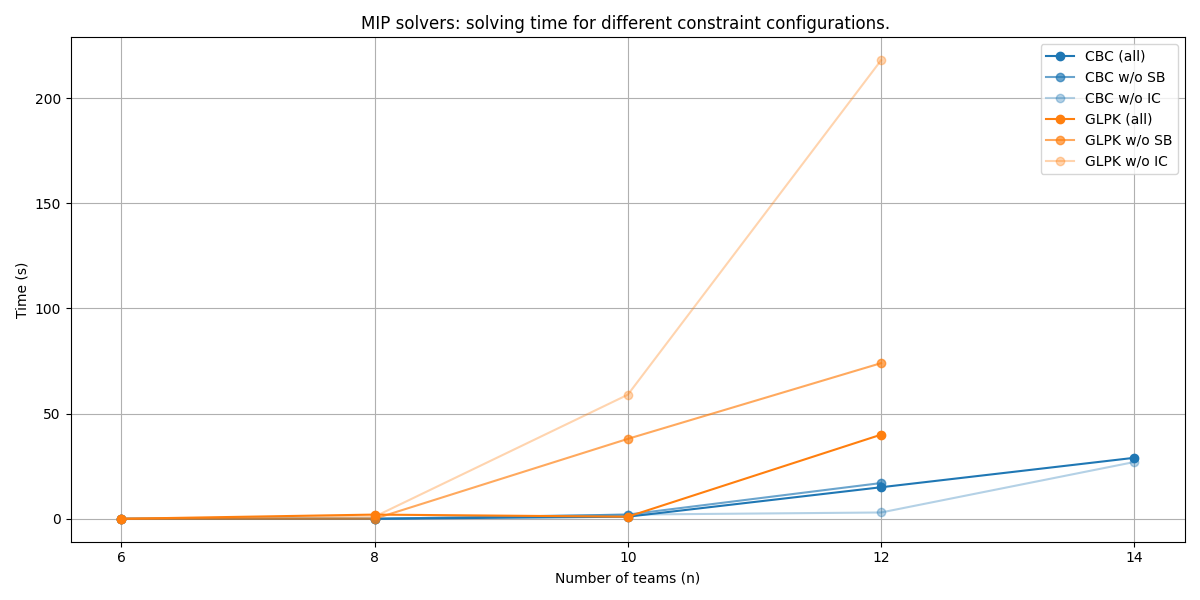
\includegraphics[width=0.8\textwidth]{mip_plot.png}
    \caption{MIP solvers: solving time for different constraint configurations.}
    \label{fig:mip_plot}
\end{figure}

\section{Conclusions}

This comparative study reveals several important insights about multi-paradigm optimization for the Sports Tournament Scheduling problem:

\begin{enumerate}    
    \item \textbf{Optional constraints impact}: The added symmetry breaking and implied constraints can be for some model beneficial, some of them having great improvements particularly noticeable with larger number of teams.
    
    \item \textbf{Encoding sensitivity}: SAT performance varies significantly with encoding choice, with bitwise encoding consistently outperforming alternatives.
    
    \item \textbf{Scalability patterns}: CP excels in optimization objectives and modeling flexibility.
\end{enumerate}

\newpage
\section*{Authenticity and Author Contribution Statement}

We declare that the work described in this report is our own and has not been copied from any other source. All external ideas, resources, or materials that have been used have been appropriately cited and referenced in the bibliography.

AI-generated content has been used in this report and it was limited to language and formulae refinement, conceptual clarification, without compromising academic integrity.

\noindent \textbf{Author Contributions:}
Both authors contributed to every model, dividing them into GitHub issues as it is showed in \url{https://github.com/leo-tasso/STS/issues?q=is%3Aissue}.


\bibliographystyle{plain}
\begin{thebibliography}{99}

\bibitem{teamsymm}
A Sport Scheduling problem example by \textit{csplib}.\\
\url{https://www.csplib.org/Problems/prob026/models/SportsScheduling.py.html}
\bibitem{tseitin}
\textit{G. S. Tseitin}, "On the complexity of derivation in propositional calculus," Studies in Constructive Mathematics and Mathematical Logic, Part II, pp. 115–125, 1968.

\end{thebibliography}

\end{document}

